\documentclass[12pt,twoside]{report}

% some definitions for the title page
\newcommand{\reporttitle}{Transfer Learning for Deep Learning Radiotherapy Planning}
\newcommand{\reportauthor}{Anton Zhitomirsky}
\newcommand{\supervisor}{Prof Ben Glocker}
\newcommand{\secondMarker}{Dr Thomas Heinis}
\newcommand{\reporttype}{MEng Individual Project}

% load some definitions and default packages
%%%%%%%%%%%%%%%%%%%%%%%%%%%%%%%%%%%%%%%%%
% University Assignment Title Page 
% LaTeX Template
% Version 1.0 (27/12/12)
%
% This template has been downloaded from:
% http://www.LaTeXTemplates.com
%
% Original author:
% WikiBooks (http://en.wikibooks.org/wiki/LaTeX/Title_Creation)
%
% License:
% CC BY-NC-SA 3.0 (http://creativecommons.org/licenses/by-nc-sa/3.0/)
% 
%
%%%%%%%%%%%%%%%%%%%%%%%%%%%%%%%%%%%%%%%%%
%----------------------------------------------------------------------------------------
%	PACKAGES AND OTHER DOCUMENT CONFIGURATIONS
%----------------------------------------------------------------------------------------
\usepackage[a4paper,hmargin=2.0cm,vmargin=1.0cm,includeheadfoot]{geometry}
\usepackage{textpos}

\usepackage[square,numbers]{natbib} % for bibliography
\usepackage[nottoc]{tocbibind} % Includes "References" in the table of contents
\bibliographystyle{unsrtnat}

\usepackage{tabularx,longtable,multirow,subfigure,caption}%hangcaption
\usepackage{fancyhdr} % page layout
\usepackage{url} % URLs
\usepackage[english]{babel}
\usepackage{amsmath}
\usepackage{graphicx}
\usepackage{scalerel}
\usepackage{dsfont}
\usepackage{epstopdf} % automatically replace .eps with .pdf in graphics
\usepackage{backref} % needed for citations
\usepackage{array}
\usepackage{latexsym}

\usepackage[pdftex,pagebackref,hypertexnames=false,colorlinks]{hyperref} % provide links in pdf
\usepackage{booktabs}
\usepackage{wrapfig}
\usepackage{caption}  % Required for \captionof
\usepackage{float} % for H option in figures
\usepackage{amssymb}
\usepackage{amsmath}
\usepackage{csquotes}
% \usepackage{subcaption} % causes a compilation error after changing back to natbib referencing... 

\hypersetup{pdftitle={},
  pdfsubject={}, 
  pdfauthor={},
  pdfkeywords={}, 
  pdfstartview=FitH,
  pdfpagemode={UseOutlines},% None, FullScreen, UseOutlines
  bookmarksnumbered=true, bookmarksopen=true, colorlinks,
    citecolor=black,%
    filecolor=black,%
    linkcolor=black,%
    urlcolor=black}

\usepackage[all]{hypcap}

%%%%%%%%%%%%%%%%%%%%%%%%%%%%%%%%%%%%%%%%%%%%%%%%%%%%%%%%%%%%%%%%%%%%%%%%%%%%%%%%
% LISTINGS ammendments
%%%%%%%%%%%%%%%%%%%%%%%%%%%%%%%%%%%%%%%%%%%%%%%%%%%%%%%%%%%%%%%%%%%%%%%%%%%%%%%%
\usepackage{listings}

\lstset
{ %Formatting for code in appendix
    language=Matlab,
    basicstyle=\footnotesize,
    % numbers=left,
    stepnumber=1,
    showstringspaces=false,
    tabsize=1,
    breaklines=true,
    breakatwhitespace=false,
    frame=single,
    columns=fullflexible,
    postbreak=\mbox{\textcolor{red}{$\hookrightarrow$}\space},
}

%\usepackage{color}
%\usepackage[tight,ugly]{units}
%\usepackage{float}
%\usepackage{tcolorbox}
%\usepackage[colorinlistoftodos]{todonotes}
% \usepackage{ntheorem}
% \theoremstyle{break}
% \newtheorem{lemma}{Lemma}
% \newtheorem{theorem}{Theorem}
% \newtheorem{remark}{Remark}
% \newtheorem{definition}{Definition}
% \newtheorem{proof}{Proof}


%%% Default fonts
\renewcommand*{\rmdefault}{bch}
\renewcommand*{\ttdefault}{cmtt}


%%% Default settings (page layout)
\setlength{\parindent}{0em}  % indentation of paragraph
\setlength{\parskip}{.3em}

% \setlength{\parindent}{0em}  % indentation of paragraph

\setlength{\headheight}{14.5pt}
\pagestyle{fancy}
\renewcommand{\chaptermark}[1]{\markboth{\chaptername\ \thechapter.\ #1}{}}
%\fancyhead[RO]{\sffamily \textbf{\thepage}} %Page no.in the right on even pages
%\fancyhead[LE]{\sffamily \textbf{\thepage}} %Page no. in the left on odd pages

\fancyfoot[ER,OL]{\thepage}%Page no. in the left on
%odd pages and on right on even pages
\fancyfoot[OC,EC]{\sffamily }
\renewcommand{\headrulewidth}{0.1pt}
\renewcommand{\footrulewidth}{0.1pt}
\captionsetup{margin=10pt,font=small,labelfont=bf}


%--- chapter heading

\def\@makechapterhead#1{%
  \vspace*{10\p@}%
  {\parindent \z@ \raggedright \sffamily
    \interlinepenalty\@M
    \Huge\bfseries \thechapter \space\space #1\par\nobreak
    \vskip 30\p@
  }}

%--- chapter heading

\def\@makechapterhead#1{%
  \vspace*{10\p@}%
  {\parindent \z@ \raggedright \sffamily
    %{\Large \MakeUppercase{\@chapapp} \space \thechapter}
    %\\
    %\hrulefill
    %\par\nobreak
    %\vskip 10\p@
    \interlinepenalty\@M
    \Huge\bfseries \thechapter \space\space #1\par\nobreak
    \vskip 30\p@
  }}

%---chapter heading for \chapter*  
\def\@makeschapterhead#1{%
  \vspace*{10\p@}%
  {\parindent \z@ \raggedright
    \sffamily
    \interlinepenalty\@M
    \Huge \bfseries  #1\par\nobreak
    \vskip 30\p@
  }}
\allowdisplaybreaks

% load some macros
% Here, you can define your own macros. Some examples are given below.

\newcommand{\R}[0]{\mathds{R}} % real numbers
\newcommand{\Z}[0]{\mathds{Z}} % integers
\newcommand{\N}[0]{\mathds{N}} % natural numbers
\newcommand{\C}[0]{\mathds{C}} % complex numbers
% \renewcommand{\vec}[1]{{\boldsymbol{{#1}}}} % vector
\newcommand{\mat}[1]{{\boldsymbol{{#1}}}} % matrix

\usepackage{pifont,mdframed}
\newenvironment{warning}
  {\par\begin{mdframed}[linewidth=1pt,linecolor=black]%
    \begin{list}{}{\leftmargin=1cm
                  \labelwidth=\leftmargin}\item[\Large\ding{43}]}
  {\end{list}\end{mdframed}\par}

\definecolor{lightgray}{gray}{0.9}

% load title page
\begin{document}
% Last modification: 2015-08-17 (Marc Deisenroth)
\begin{titlepage}

    \newcommand{\HRule}{\rule{\linewidth}{0.5mm}} % Defines a new command for the horizontal lines, change thickness here
    
    %----------------------------------------------------------------------------------------
    %	LOGO SECTION
    %----------------------------------------------------------------------------------------
    
    
\includegraphics[width = 4cm]{../figures/imperial.pdf}\\[0.5cm] 
    
    \center % Center everything on the page
     
    %----------------------------------------------------------------------------------------
    %	HEADING SECTIONS
    %----------------------------------------------------------------------------------------
    
    \textsc{\LARGE \reporttype}\\[1.5cm] 
    \textsc{\Large Department of Computing}\\[0.5cm] 
    \textsc{\large Imperial College of Science, Technology and Medicine}\\[0.5cm] 
    
    %----------------------------------------------------------------------------------------
    %	TITLE SECTION
    %----------------------------------------------------------------------------------------
    
    \HRule \\[0.4cm]
    { \huge \bfseries \reporttitle}\\ % Title of your document
    \HRule \\[1.5cm]
     
    %----------------------------------------------------------------------------------------
    %	AUTHOR SECTION
    %----------------------------------------------------------------------------------------
    
    \begin{minipage}{0.4\textwidth}
    \begin{flushleft} \large
    \emph{Author:}\\
    \reportauthor % Your name
    \end{flushleft}
    \end{minipage}
    ~
    \begin{minipage}{0.4\textwidth}
    \begin{flushright} \large
    \emph{Supervisor:} \\
    \supervisor % Supervisor's Name
    \end{flushright}
    \end{minipage}\\[4cm]
    
    
    
    
    %----------------------------------------------------------------------------------------
    
    
    %----------------------------------------------------------------------------------------
    %	DATE SECTION
    %----------------------------------------------------------------------------------------
    
    {\large \today} % Date, change the \today to a set date if you want to be precise
    
    
    \vfill % Fill the rest of the page with whitespace
    Submitted in partial fulfillment of the requirements for the \degreetype~of Imperial College London
    
    \end{titlepage}
    

% page numbering etc.
\pagenumbering{roman}
\clearpage{\pagestyle{empty}\cleardoublepage}
\setcounter{page}{1}
\pagestyle{fancy}

% \cleardoublepage
%%%%%%%%%%%%%%%%%%%%%%%%%%%%%%%%%%%%
% \section*{Acknowledgments}
% Comment this out if not needed.

% \clearpage{\pagestyle{empty}\cleardoublepage}

%%%%%%%%%%%%%%%%%%%%%%%%%%%%%%%%%%%%

\begin{abstract}\label{sect:abstract}
    Cervical cancer remains as one of the top cancerous diseases to affect women. To treat it, Oncologists plan a contour for therapy after obtaining 3D contrasting images of soft-tissue organs at risk and tumorous areas. 
  
    Auto-segmentation differs from Auto-contouring tasks due to lacking clinical knowledge surrounding the location of the cancer and biological spreading patterns. Instead of trivially contouring visible macroscopic tumour masses on a scanned patient, a clinician requires also to adjust for microscopic spreads and finally error margin spreads. This target volume should aim to treat the disease in one-shot and not affect any organs-at-risk.
    
    The scientific community has tried to automate this task using current architectural standards such as CNNs or U-Net based algorithms. However, no studies yet consider Transfer Learning as an approach to solving this issue. This report investigates this architectural challenge to contribute to the total pool of deep learning auto-segmentation models in a communal effort to save resources of medical institutions.
  
    You can find the most up-to-date version of the report \href{https://github.com/AntonZhitomirsky/radiotherapy/blob/main/report/interim/interim.pdf}{\textit{here}}.
  
  \end{abstract}
  
%%%%%%%%%%%%%%%%%%%%%%%%%%%%%%%%%%%%
%--- table of contents
\fancyhead[RE,LO]{\sffamily {Table of Contents}}
\tableofcontents
  
% \clearpage{\pagestyle{empty}\cleardoublepage}

%%%%%%%%%%%%%%%%%%%%%%%%%%%%%%%%%%%%
\chapter{Introduction}\label{sect:intro}

\pagenumbering{arabic}
\setcounter{page}{1}
\fancyhead[LE,RO]{\slshape \rightmark}
\fancyhead[LO,RE]{\slshape \leftmark}

\section{Clinical Context}



In 2017, Cervical Cancer accumulated 530,000 new cases annually, with 270,000 deaths, making it the fourth most common malignancy diagnosed in women worldwide~\cite{cervical-cancer-epidemic}. A common treatment mechanism involves radiation therapy which targets cancerous cells in a clinically defined target area with beams of high energy (Section~\ref{sect:radiotherapy}). This treatment is tedious, as it is estimated that an oncologist needs 90-120 min to delineate target areas for radiotherapy~\cite{LIU2020184}.

Radiotherapy has become a great option due to high resolution X-ray or CT scans which produce high contrasting images of the damaged and surrounding soft tissue~\cite{radiotherapy-basic-concepts}. Physicians then use this 3D scan to plan a target volume for the radiation therapy surrounding the tumor in hopes of killing it and not damaging the surrounding tissue.

Areas are therefore constructed based on an Oncologist knowledge about the particular cancer to determine target structures, structures we need to protect (organs-at-risk), and areas where each particular cancer is likely to spread to~\cite{AMLART-data}. These areas are delineated onto a patient scan and used as a radiotherapy target used for treatment.

Accurate scans have been provided to see if an AI model can learn cervical cancer CTV patterns adjacent to clinical knowledge and oncologist prior knowledge. Training models which produce substructures required for radiotherapy target volumes would overall save time and improve consistency within the radiotherapy planning process~\cite{AMLART-data}.

\section{Current Solutions}\label{sect:current-solutions}

The problem of automatic delineation of tumours in a patient is not a new concept unfamiliar to the scientific community. From 2016 to 2020 the number of deep-learning in radiotherapy publications has grown from 1,001 to 3,653~\cite{Lin2021-oz}. Therefore, there exist many proposals and solutions to this problem for cancerous tumours across the body. This also includes research projects focused specifically on cervical cancer and radiotherapy auto-contour planning. By conducting a accrual of literature across PubMed with the search string

\begin{lstlisting}
  ``radiotherapy'' AND ``contour'' AND (``cervix'' OR ``cervical'') AND ``cancer'' AND (``Deep Learning'' OR ``DeepLearning'' OR ``Machine Learning'' OR ``ML'' OR ``Artificial Intelligence'' OR ``AI'' OR ``Computer assisted'')  
\end{lstlisting}

6 key papers published between the span of 2020 to 2021 were selected as most relevant for this project~\cite{Samarasinghe2021-ps,Lin2021-oz,Sartor2020-et,LIU2020184,Rhee2020-ms,LIU2020172}. These papers proposed novel ideas on how to solve image segmentation problems. Some noteworthy networks included Convolutional Neural Networks (Section~\ref{sect:CNNs}), 2D and 3D U-Net adaptations (Section ~\ref{sect:u-net} and~\ref{sect:nnu-net}), V-Nets and DeepMedic models, with the most common approach being the U-Net approach according to a clinical survey on the topic in 2021~\cite{Samarasinghe2021-ps}. The methods in these papers will be further discussed in Chapter~\ref{sect:background}.

\section{Motivation}\label{sect:motivation}

\subsubsection{Healthcare Crisis}

Healthcare centres are experiencing high demand with low availability for all types of cancer. In England, waiting times are getting worse each month, with over a third of cancer patients (60,000) waiting beyond the 62-day target, and 10,000 patients waiting over 104 days according to a radiotherapy manifesto in 2022 \href{https://radiotherapy.org.uk/wp-content/uploads/2022/11/APPGRadiotherapy_Manifesto-Update_2022.pdf}{\textit{Manifesto link (shall i put in bibliography?)}}. 

This wait is partially due to the time consuming nature of treatment plans, with manual segmentation performed by a professional oncologist taking 90-120 minutes~\cite{LIU2020184,Sartor2020-et} while always requiring optimization of radiotherapy placement to avoid oragns-at-risk~\cite{Samarasinghe2021-ps}.

Furthermore, more resources can be partitioned into other departments by developing software to aid with cancer treatments. A study found that the scale-up of radiotherapy capacity in 2015-35 from current levels `could lead to saving of 26.9 million life-years in low-income and middle-income countries over the lifetime of the patients who received treatment'~\cite{expanding-global-access-to-radiotherapy}.

\subsubsection{Current Tools}

Unfortunately, there is a difference between auto-contouring and auto-segmentation. For our case we cannot use models such as TotalSegmentator (Section \ref{sect:totalseg}). TotalSegmentator has learnt form many samples to delineate 117 classes of objects in the human body, such as bones, a large subset of significant organs and veins~\cite{totalsegmentor-git}. Our case involves delineating a PTV, which is a significant challenge because it involves meta-information which is not visible on a CT scan, and therefore is not a trivial task of tracing around the visible contours of a tumour, but more so about adding sufficient padding to account for the microscopic spread of the tumour not visible to the scanner.

Since wrong or inaccurate contours constitute the highest factors for failure of treatment~\cite{Rhee2020-ms} current tools that are not bespoke for the task are therefore poor candidates for practical use.

\subsubsection{Research Gap}

The current literature makes great use of modern concepts stemming from the discovery of CNN models for auto-segmentation for radiotherapy planning. However, all papers assume a good sample size which represents the overall population of people under the same conditions. This is not practical in a general case, for instance: hospitals may only have the data for their in-house patients, teams operate on a niche areas and therefore have a smaller sample size, affected area scans are not standardized and vary between organizations which may promote the `garbage in, garbage out' philosophy, and finally varying degrees of catastrophe levels pertaining to the sensitivity of the organs at risk (Section~\ref{sect:contour-planning}) surrounding the tumour (radiotherapy in the pelvis vs radiotherapy in the brain).

\subsubsection{Summary}

We therefore propose a solution that can be applied to groups with specific niche rules and small sample sizes. This Transfer Learning approach (Section \ref{sect:transfer-learning}) aims to leverage other trained models with great performance and lift low-level features to use in our case. This will also fill the literature gap which hasn't considered solving the auto-contouring for radiotherapy planning volumes, as a PubMed search querying publications with mentions of transfer learning returned no relevant matches.

\section{Outline of Report}\label{sect:outline-of-report}

The structure of this report will take the reader of a reasonable programming background through the project such that they might be able to reconstruct the outcome themselves. It is expected of the reader to understand the concept of Machine Learning and an intuition surrounding Computer Vision.

Firstly Chapter~\ref{sect:background} discusses the clinical context (Section~\ref{sect:clinical-context}) from which the idea for this project originates. We further construct the background knowledge for the current Computer Vision methodologies which exist to solve segmentation based issues (Section~\ref{sect:image-segmentation}). This will lead into currently pre-trained models (Section~\ref{sect:existing-auto-segmentation-methods}) and their application in a Transfer Learning setting (Section~\ref{sect:transfer-learning}).

% With collaboration from the Royal Marsden Hospital they have provided this project with a set of data (Chapter~\ref{sect:data}) with which the remainder of this project is trained upon, the usage concerns have been evaluated through the Ethics chapter (Chapter~\ref{sect:ethics}). We discuss what constitutes an accurate segmentation and reason about evaluation metrics to provide an outlook on the models performance (Chapter~\ref{sect:evaluation-metrics}).

% Finally, Chapter~\ref{sect:proposal} contains details surrounding the proposition of this project. We establish base-line results (Section~\ref{sect:baseline-results}) such that we may see that our future implementation will supersede the common implementation. Currently, for the interim report the proposition lays bare, but will be slowly added throughout the course of the project.

%%%%%%%%%%%%%%%%%%%%%%%%%%%%%%%%%%%%
\chapter{Background}\label{sect:background}

\section{Clinical Context}\label{sect:clinical-context}

This section will provide a baseline understanding of the clinical context for developing a tool to help segment tumours in patients with cervical cancer. Considering the unfortunate high frequency of cancers developing in people across the globe~\cite{cervical-cancer-epidemic}, the idea for developing a model to help segment cancers has long been in the scope for many researchers.

\subsection{Cervical Cancer}\label{sect:cervical-cancer}

In 2017, Cervical Cancer accumulated 530,000 new cases annually, with 270,000 deaths, making it the fourth most common malignancy diagnosed in women worldwide~\cite{cervical-cancer-epidemic}. A common treatment mechanism involves radiation therapy which targets cancerous cells in a clinically defined target area with beams of high energy (Section~\ref{sect:radiotherapy}). This treatment is tedious, as it is estimated that an oncologist needs 90-120 min to delineate target areas for radiotherapy~\cite{LIU2020184}.

This time consuming nature of studying each patient makes treating cancers a time consuming endeavour which is particularly threatening when time is not on the patients side. Death from Cervical Cancer involves significant pain and suffering for the patients who cannot receive urgent treatment~\cite{cervical-cancer-epidemic}. This is particularly a problem in mid-low income countries with approximately 85\% of cases of cervical cancer occurring, making them have 18 times the death rates of high-income countries~\cite{cervical-cancer-epidemic}. 

\subsection{Radiotherapy}\label{sect:radiotherapy}

Radiation therapy is a treatment option for cancer treatment. In 2012, approximately 50\% of all cancer patients received radiation therapy, with an additional 40\% involving curative treatment~\cite{radiotherapy-advances}. 

Physicians abuse the physical properties of radiation to damage the genetic material of cells and block their ability to cause further damage to a patient~\cite{radiotherapy-advances}. Importantly for our cause, radiation damages intercellular molecules leading to degradation and stopping a cells ability to divide, leading to interphase death. Alternatively, radiation may cause a ``mitotic catastrophe'' causing a cell to die of a proliferative death~\cite{cell-death}. 

\subsection{Contour Planning}\label{sect:contour-planning}

Radiotherapy has become a great option due to high resolution X-ray or CT scans which produce high contrasting images of the damaged and surrounding soft tissue~\cite{radiotherapy-basic-concepts}. Physicians then use this 3D scan to plan a target volume for the radiation therapy surrounding the tumor in hopes of killing it and not damaging the surrounding tissue.

\subsubsection{Process}

This begins with the high contrasting image of the tumour area. In a clinical setting, an Oncologist will use knowledge about the particular cancer to determine target structures, structures we need to protect (organs-at-risk), and areas where each particular cancer is likely to spread to~\cite{AMLART-data}. 

The first area defined from the scan is the Gross Target Volume (GTV). This macroscopic delineated area is the visible tumour area on the scan and contains a high probability of containing the tumour. Secondly, the Clinical Target Volume (CTV) is derived to account for potential microscopic spread. This will be an area at least as big as the tumor area segmented in the GTV with an optional margin surrounding it containing a 'rind' of non-zero probability of tumour spread. Lastly, the Primary Tumour Volume (PTV) contains residual geometric uncertainties and safety margins surrounding the CTV ensuring the radiotherapy dose is actually delivered to the CTV~\cite{tumor-delineation,defining-target-volumes,Lin2021-oz,personalised-PTV-strategies}. These target volumes also constantly consider critical normal tissue structures which need to be preserved during irradiation. These are referred to as organs-at-risk (ORs). In some specific circumstances, it is necessary to add a margin analogous to the PTV margin around an OR to ensure that the organ cannot receive a higher-than-safe dose; this gives a planning organ at risk volume~\cite{defining-target-volumes}.

\subsubsection{A tangent on Accuracy}

The CTV volumes may vary between clinicians as there is no internationally agreed guidelines. As a very time consuming process which high variability it therefore suffers from a lot of inter and intra-observer variability~\cite{Lin2021-oz}. However, the data provided has been standardized as a gold standard, see Section~\ref{sect:data}.

The PTV volume is an additional step which provides a margin of protection surrounding the CTV. One might think that a CTV step is the final step in clinical trials as it defines the most tight volume surrounding the cancerous site, however, geometric errors are impossible to eliminate. This includes short-term organ movement, voxel size and slice resolution, and possibility of relative movement of structure of reference and the tumour~\cite{VANHERK200452}

\section{Existing Auto-Segmentation Methods}\label{sect:existing-auto-segmentation-methods}

\subsection{Total Segmentator}\label{sect:totalseg}

TotalSegmentator~\cite{totalsegmentor-paper} is a model that was developed be a very robust segmentation tool. It has been trained on 1204 CT examinations and once more on 4004 whole-body CT examinations to investigate age dependent volume and attenuation changes. TotalSegmentator has learnt a robust model for delineating 117 classes of objects in the human body, such as bones, a large subset of significant organs and veins~\cite{totalsegmentor-git}

\begin{wrapfigure}{L}{0.5\textwidth}
  \centering
  \includegraphics*[width=0.5\textwidth]{../figures/AnnotationWorkflow.png}
\end{wrapfigure} 

It uses an iterative learning approach.

(1) After manual segmentation of the first 5 patients was completed, (2) a preliminary nnU-Net was trained, (3) and its predictions were manually refined, if necessary. (4) Retraining of the nnU-Net was performed after (5) reviewing and refining 5 patients, 20 patients, and (6) 100 patients.

In the end, all 1204 CT examinations had annotations that were manually reviewed and corrected whenever necessary. These final annotations served as the ground truth for training and testing. The model was trained on the dataset of 1082 patients, validated on the dataset of 57 patients and tested on the dataset of 65 patients. This final model was independent of the intermediate models trained during the annotation workflow, which reduced bias in the test set to a minimum. Using completely manual annotations in the test set would have introduced a distribution shift and thus greater bias~\cite{totalsegmentor-paper}.

% The model uses an nnU-Net (Section~\ref{sect:nnu-net}) because of its ability yo automatically configure hyperparameters based on the dataset characteristics. 

TotalSegmentator is a model which encountered some issues with the dataset that may have impeded its performance. Firstly, some patients had ribs missing, which a clinician would typically count from top/bottom to identify them; however, on some scans these weren't visible, much like in our case, we are missing overies. These have been attributed to reasons for low performance for these structures, which warns us; our dataset contains many abnormalities according to the descriptions of each patient (Section~\ref{sec:data-notes}).

\subsection{UniverSeg}\label{sect:universeg}



\subsection{SAM}\label{sect:sam}

TODO: maybe replace with medical SAM paper.

\section{Current Limitations}\label{sect:limitations}

% The approaches listed in Section~\ref{sect:image-segmentation} and models discussed in Section~\ref{sect:existing-auto-segmentation-methods} are great approaches for most image segmentation applications. We've seen the advancements of CNNs to tackle the intractable nature of fully connected neural network, and the advancements in segmentation models in the U-Net. Furthermore, these techniques have been used to train robust models in medicine such as those presented in Section~\ref{sect:existing-auto-segmentation-methods}. 

However, our problem is not accurately solved with the methods mentioned. This is due to a handful of independent details which require more careful planning and engineering.

\subsection{Data Size}\label{sect:solving-the-problem-data-size}

The data quantity supplied is a limiting factor for creating a robust model. We are given 100 labeled data elements across 5 classes. Without vast collection of knowledge, it is hard for an application to create a model which generalizes well to the total population, especially in a very specific and bespoke use case as radiotherapy planning for cervical cancer.

\subsection{Bespoke Application}\label{sect:solving-the-problem-bespoke-application}

Another issue lies in the bespoke nature of this application. Most pre-trained networks currently run segmentation on structures are that are more obvious in a given image modality. For instance, TotalSegmentator has learnt a robust model for delineating 117 classes of objects in the human body, such as bones, a large subset of significant organs and veins~\cite{totalsegmentor-git}. Our application is unique because the PTV often includes a margin surrounding the visible tumour on the scan, which is different to other approaches which outline the boundaries of structures.

\section{Transfer Learning}\label{sect:transfer-learning}

Transfer Learning uses knowledge that has been obtained from one task, and uses it as a starting point for learning a new task. It is therefore a useful solution to the problems identified in Section~\ref{sect:limitations} because of the transferable knowledge features for similar domains  and its proven success in generalizing features is trained properly.

The intuitive reason why transfer learning works is because in the early layers of deep learning, the model learns very low-level features. At this scale, the initial data-set or the cost function doesn't matter because a model working on the same problem but with different initialization will learn similar low-level features. This allows transferral because the (large/sufficiently sized) input dataset is abstracted in the set low-level features which can instead be transferred. Then, the later layers are more specialized to a particular task~\cite{deep-learning-book}. It is similar to seeing the distribution in the training data change and transferring knowledge across domains~\cite{survey-on-transfer-learning}.

\begin{figure}[H]
  \centering
  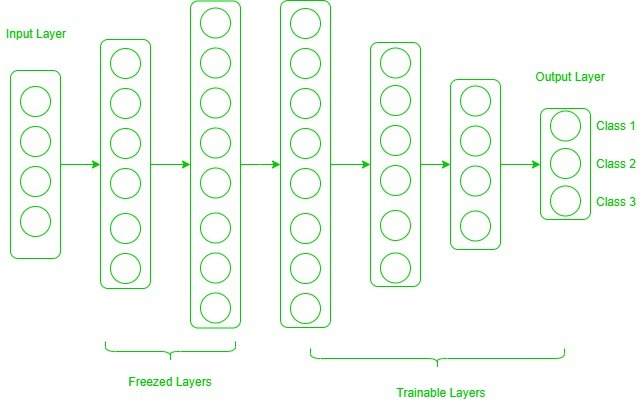
\includegraphics[width=0.7\linewidth]{../figures/Frozen-layers.jpg}
  \caption{Early layers learn low-level features for similar domains, and during transfer of knowledge, these layers are frozen and the trainable layers are appended and weights are only updated for this layer~\cite{geeks-transfer-learning}}
 \label{fig:frozen-layers}
\end{figure}

Transfer Learning has the potential to: improve initial performance using only the transferred knowledge before nay further learning is done, improve the time it takes to fully learn the target task given the transferred knowledge, and improve the final performance all when compared to initial benchmarks without transfer~\cite{torrey-handbook}. It has also been found to work in medical contexts as well, where, for 332 abdominal liver CT scans, transfer learning generally improved weight initialization and resulted in faster convergence providing stronger and more robust representation~\cite{liver-lesion-via-transfer-learning}

Transfer Learning has been seen to prevent overfitting in domains where data volume is low and where generality without overfitting is hard to come by. This is because the model has already learnt features that are likely to be useful in the second task~\cite{geeks-transfer-learning}. 

However, generalization is not a guarantee, as overfitting is still possible if the model is fine-tuned too much on the second task, as it may `learn task-specific features that do not generalize well to new data'~\cite{geeks-transfer-learning}. In our case, our target dataset is small, but similar to the base network dataset. Here, we may overfit because fine-tune the pre-trained network with the target dataset may not generalize to the global population. If instead we attempt to transfer a task with different base network dataset, then using high-level features of the pre-trained model will not be useful~\cite{geeks-transfer-learning}.

%%%%%%%%%%%%%%%%%%%%%%%%%%%%%%%%%%%%

% \chapter{Data}\label{sect:data}

% The data is acquired during a CT scan (Section~\ref{sec:data-ct-scan}) and presented as a set of \texttt{NIfTI} (Section~\ref{sec:data-file-format}) files provided by the Royal Marsden Hospital. The data is of 100 patients each with a variant of cervical cancer. We have obtained from the hospital a spreadsheet with additional notes about each patient which may be useful in training and debugging (Section~\ref{sec:data-notes}). Finally, this data is labelled into 5 different classes as a binary segmentation problem (Section~\ref{sec:data-delineation-classes}). Included is a set of 10 hold-out data items, which are patients with only the raw CT scan with no labels.

% Delineated labelled data have been labelled consistently by the provider to improve chances that an AI model can learn cervical cancer CTV patterns~\cite{AMLART-data}.

% \section{CT scan}\label{sec:data-ct-scan}

% Before we consider other aspects of the data it is helpful to consider the context from which it was extracted and therefore what we might expect to see. This data is in CT scan, and so will be the focus, although there exist other imaging modalities such as Magnetic Resonance Imaging (MRI) and others.

% A CT Scan is an X-ray study, where a series of rays are rotated around a specified body part, and computer-generated cross-sectional images are produced~\cite{file-formats}. The granularity or image slice thickness is decided by the operator or physician and ranges from 1mm to 10mm. Whilst the scanner rotates the X-ray tube the patient is slowly moved up or down in the table to produce different cross-section images.

% We therefore expect to receive a representation of the internal structure or functions of an atomic region in the form of an array of voxels. A voxel represents the value on a grid in three-dimensional space and is decided by the physician once they establish the slice thickness.

% This data format is contrary to natural images, where the pixel values vary from 0 to 255. In a CT scan, readings are represented by the Hounsfield Scale~\cite{diagnostic-radiology-physics}. This scale is a quantitative scale for describing radiodensity where the image intensity reflects tissue type; each voxel intensity refers to specific tissue composition. This means for our purposes data normalization is not necessary, becuase intensities are not relative, and the model would not suffer from reading raw unnormalized data. Therefore, there are typical value ranges for different tissue types like fat being between $-100$ to $-80$ and muscle from $+10$ to $+40$. Since the minimum bit depth for such measurements is 12, downscaling to an 8 bit greyscale image may fool an observer about the detail of the scan, however, information is represented in full resolution.

% \section{File Format}\label{sec:data-file-format}

% The files are stored in a \texttt{.nii} file format which defines a style of image called the `Neuroimaging Informatics Technology Initiative' (NIfTI)~\cite{file-formats}. It serves as a lightweight alternative to other formats such as DICOM and eliminates ambiguity from spatial orientation information~\cite{dicom-to-nifti-conversion}.

% The file has a fixed-size header which stores information about the data collected. Table~\ref{tab:nifti-header} summarizes some key attributes of the header. All other attributes not listed are handled by the SimpleITK library~\cite{SimpleITK-paper} which we use to read and manipulate the data in this project. The library defines the image as a set of points in a grid occupying a physical region in space as defined by this metadata, and therefore is influenced by the origin, size, spacing and so on.

% \begin{table}[ht]
%   \centering
%   \begin{tabular}{>{\raggedright}p{1.5cm}p{8cm}p{4cm}}
%     \toprule
%     \textbf{Name} & \textbf{Meaning}                                                                          & \textbf{Value example} \\
%     \midrule
%     dim           & Image dimension                                                                           & 3 512 512 193 1 1 1 1  \\
%     bitpix        & Number of bits per voxel                                                                  & 32                     \\
%     pixdim        & The grid spacing (voxel size) and optionally time interval                                & 0 1.3 1.3 2.5 0 0 0 0  \\
%     xyzt\_units   & indicates units of pixdim and defined in the C header, e.g. \texttt{NIFTI\_UNITS\_MM = 2} & 2                      \\
%     \bottomrule
%   \end{tabular}
%   \caption{Description of NIfTI header parameters relevant to this project~\cite{dicom-to-nifti-conversion, nifti-headers, nifti-data-format}. Example values are taken from patient id:075.}
%  \label{tab:nifti-header}
% \end{table}

% \section{Notes}\label{sec:data-notes}

% The notes contain information about each of the 100 labelled data pairs~\cite{AMLART-data}. This information can be helpful in debugging or troubleshooting. It also provides a good warning regarding the variability of the data. In particular some aspects to note are summarized in Table~\ref{tab:notes-summary}.

% \begin{table}[ht]
%   \centering
%   \begin{tabular}{>{\raggedright}p{3cm}p{6cm}p{6cm}}
%     \toprule
%     \textbf{Patient ID} & \textbf{Comment}                                                                                           & \textbf{Concern}                                                                                \\
%     \midrule
%     zzAMLART003         & ``no GTVp''                                                                                                & Some scans contain no visible tumour, but we still draw a CTV                                   \\
%     \midrule
%     zzAMLART017         & ``only scanned bottom of kidneys''                                                                         & We should be cautious of variability of width scope given in our source data                    \\
%     \midrule
%     zzAMLART017         & ``missing left kidney''                                                                                    & Unusual body anatomy might trip up the model, mentioned elsewhere are also                      \\
%     \midrule
%     zzAMLART041         & ``extra slices''                                                                                           & variability in voxels or quantity may require data pre-processing to eliminate data uncertainty \\
%     \midrule
%     zzAMLART055         & ``no contrast - hard to see LNs. NG tube in situ. posterior renal vein. small parametrium and low uterus'' & An edge case like this will require more thought                                                \\
%     \bottomrule
%   \end{tabular}
%   \caption{A few captivating notes about each patient and why it might be concerning}
%  \label{tab:notes-summary}
% \end{table}

% There exist note entires for the majority of the 100 patients which weren't shown in Table~\ref{tab:notes-summary}. Regardless, these notes are helpful to identify what type of pre-processing we must do in order to fully address some differences between patients. The concern is to not overfit on the 'normal' cases but also generalize and engineer a solution that is also open-minded to extreme or poorly captured cases; there is a vast variability in the anatomy of patients which makes computer vision tasks more challenging.

% \section{Delineation classes}\label{sec:data-delineation-classes}

% The clinicians at the Royal Marsden Hospital have provided segmentation labels for 5 high-priority classes of interest. These are the Bladder, Anorectum, CTVn, CTVp, and Parametrium.

% \subsection{Organs At Risk}\label{sec:data-organs-at-risk}

% \begin{figure}[H]
%   \centering
%   \subfigure[Axial]{
%     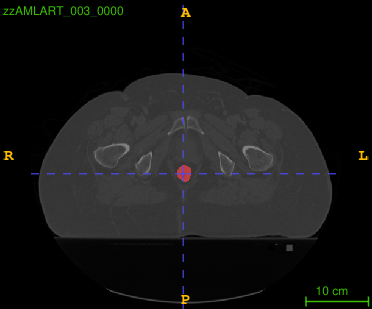
\includegraphics[width=0.3\textwidth]{../figures/PatientStructureExamples/Anorectum_003/Axial.png}
%    \label{fig:example-anorectum-axial}
%   }
%   \subfigure[Coronal]{
%     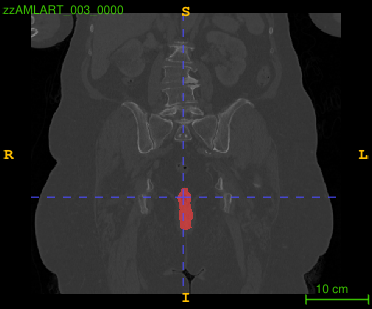
\includegraphics[width=0.3\textwidth]{../figures/PatientStructureExamples/Anorectum_003/Coronal.png}
%    \label{fig:example-anorectum-coronal}
%   }
%   \subfigure[Sagittal]{
%     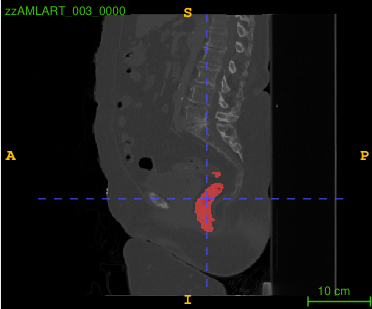
\includegraphics[width=0.3\textwidth]{../figures/PatientStructureExamples/Anorectum_003/Sagittal.png}
%    \label{fig:example-anorectum-sagittal}
%   }
%   \vspace{1em}
%   \subfigure[Axial]{
%     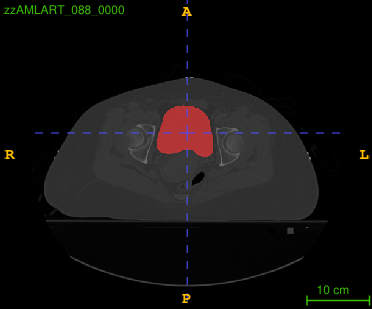
\includegraphics[width=0.3\textwidth]{../figures/PatientStructureExamples/Bladder_088/Axial.png}
%    \label{fig:example-bladder-axial}
%   }
%   \subfigure[Coronal]{
%     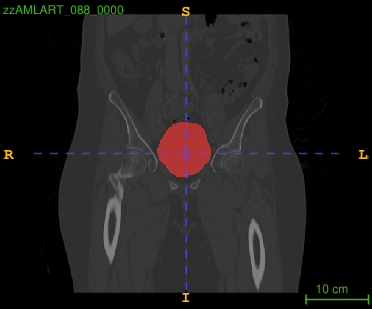
\includegraphics[width=0.3\textwidth]{../figures/PatientStructureExamples/Bladder_088/Coronal.png}
%    \label{fig:example-bladder-coronal}
%   }
%   \subfigure[Sagittal]{
%     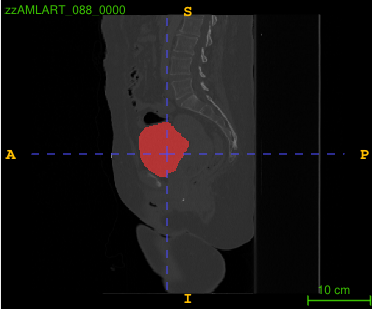
\includegraphics[width=0.3\textwidth]{../figures/PatientStructureExamples/Bladder_088/Sagittal.png}
%    \label{fig:example-bladder-sagittal}
%   }
%   \caption{Views of a segmented (in red) Anorectum (\ref{fig:example-anorectum-axial}-\ref{fig:example-anorectum-sagittal}) and Bladder (\ref{fig:example-bladder-axial}-\ref{fig:example-bladder-sagittal}) of an arbitrary patient}
% \end{figure}

% An organ at risk is an organ which has a substantial probability of being within the PTV despite being healthy. Any areas that are created around the area should actively avoid these organs because by overlapping with them we risk complicating the treatment and compromising the health of functioning organs.

% Many anatomies have been provided in the risk categories, however, in particular we have been supplied with contours for the Bladder (Figure~\ref{fig:example-bladder-axial}-\ref{fig:example-bladder-sagittal}) and the Anorectum (Figure~\ref{fig:example-anorectum-axial}-\ref{fig:example-anorectum-sagittal}). In particular, clinicians have identified that the Bladder may overlap with the CTVn (Section~\ref{sec:data-CTVn}) and the Parametrium (Section~\ref{sec:data-Parametrium}).

% \subsection{CTVp}\label{sec:data-CTVp}

% \begin{figure}[H]
%   \centering
%   \subfigure[Axial]{
%     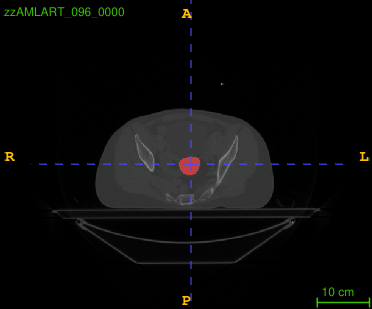
\includegraphics[width=0.3\textwidth]{../figures/PatientStructureExamples/CTVp_096/Axial.png}
%    \label{fig:example-CTVp-axial}
%   }
%   \subfigure[Coronal]{
%     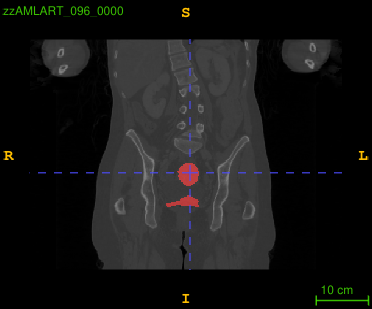
\includegraphics[width=0.3\textwidth]{../figures/PatientStructureExamples/CTVp_096/Coronal.png}
%    \label{fig:example-CTVp-coronal}
%   }
%   \subfigure[Sagittal]{
%     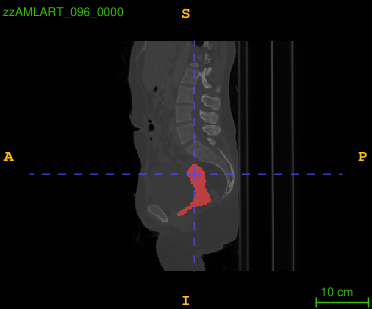
\includegraphics[width=0.3\textwidth]{../figures/PatientStructureExamples/CTVp_096/Sagittal.png}
%    \label{fig:example-CTVp-sagittal}
%   }
%   \caption{Views of a segmented (in red) CTVp of an arbitrary patient}
%  \label{fig:example-CTVp}
% \end{figure}

% The CTVp stands for the Primary Clinical Target Volume, see the example at Figure~\ref{fig:example-CTVp}. This is the CTV where there may be local microscopic spread (uterus, cervix, upper vagina, primary tumour)~\cite{AMLART-data}. This is the area that contains the tumour.

% This isn't by any means an organ in a body, but rather an area comprised of other components formed by joining other structures together. The CTVp is an area defined in Equation~\ref{eq:ctvp}.

% \subsection{CTVn}\label{sec:data-CTVn}

% \begin{figure}[H]
%   \centering
%   \subfigure[Axial]{
%     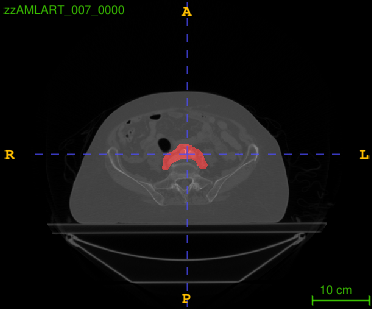
\includegraphics[width=0.3\textwidth]{../figures/PatientStructureExamples/CTVn_007/Axial.png}
%    \label{fig:example-CTVn-axial}
%   }
%   \subfigure[Coronal]{
%     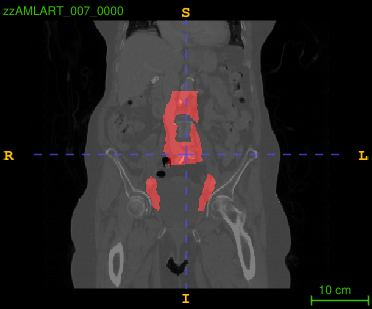
\includegraphics[width=0.3\textwidth]{../figures/PatientStructureExamples/CTVn_007/Coronal.png}
%    \label{fig:example-CTVn-coronal}
%   }
%   \subfigure[Sagittal]{
%     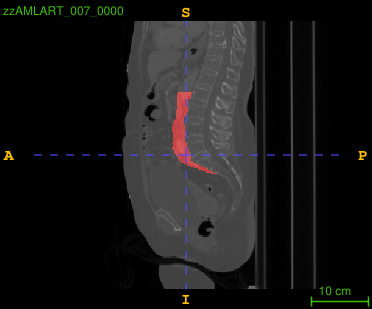
\includegraphics[width=0.3\textwidth]{../figures/PatientStructureExamples/CTVn_007/Sagittal.png}
%    \label{fig:example-CTVn-sagittal}
%   }
%   \caption{Views of a segmented (in red) CTVn of an arbitrary patient}
%  \label{fig:example-CTVn}
% \end{figure}

% The CTVn stands for Nodal Clinical Target Volume, see the example at Figure~\ref{fig:example-CTVn}. This is the CTV where there may be microscopic spread to lymph nodes. It is drawn based on set margins around pelvic blood vessels and includes pelvic lymph nodes, common iliac lymph nodes and para-aortic lymph nodes~\cite{AMLART-data}.

% Similarly to CTVp, this is a compound area with three groups of lymph nodes. In clinical practice, the number of these groups included in the CTV varies in each patient, depending on how advanced the disease is. Pathological lymph nodes (GTVn) are also included. The CTVn is an area defined in Equation~\ref{eq:ctvn}.

% \subsection{Parametrium}\label{sec:data-Parametrium}

% \begin{figure}[H]
%   \subfigure[Axial]{
%     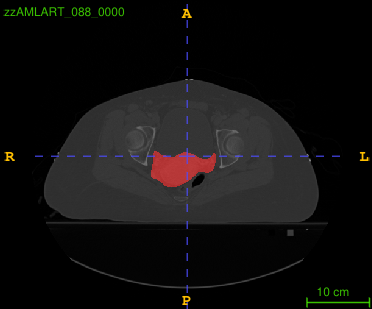
\includegraphics[width=0.3\textwidth]{../figures/PatientStructureExamples/Parametrium_088/Axial.png}
%    \label{fig:example-Parametrium-axial}
%   }
%   \subfigure[Coronal]{
%     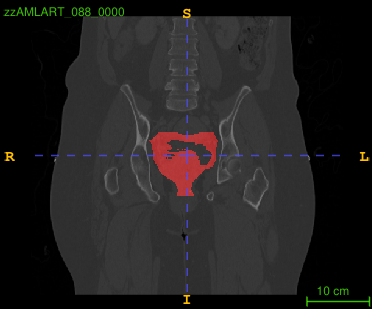
\includegraphics[width=0.3\textwidth]{../figures/PatientStructureExamples/Parametrium_088/Coronal.png}
%    \label{fig:example-Parametrium-coronal}
%   }
%   \subfigure[Sagittal]{
%     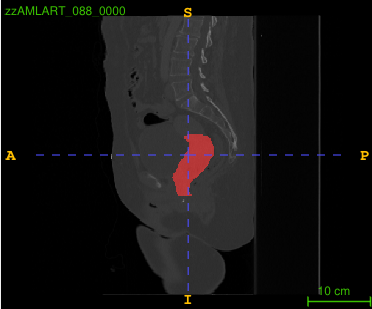
\includegraphics[width=0.3\textwidth]{../figures/PatientStructureExamples/Parametrium_088/Sagittal.png}
%    \label{fig:example-Parametrium-saggital}
%   }
%   \caption{Views of a segmented (in red) Parametrium of an arbitrary patient}
%  \label{fig:example-Parametrium}
% \end{figure}

% The Parametrium (or Paravagina) is the tissue surrounding the cervix/vagina - at risk of local spread, see Figure~\ref{fig:example-Parametrium}. Drawn as a complete structure and editing back to the level of vagina to be included~\cite{AMLART-data}.

% \section{Establishing Rules for Structures}\label{sec:data-delineation-rules}

% \begin{minipage}{0.5\textwidth}
%   \subsubsection{Notation of Structures}
%   \begin{enumerate}
%     \item Let the Anorectum be denoted as $A$
%     \item Let the Bladder be denoted as $B$
%     \item Let the Cervix be denoted with $C$
%     \item Let the CTVn be denoted with $C_n$
%     \item Let the CTVp be denoted with $C_p$
%     \item Let the GTVp be denoted with $G_p$
%     \item Let the GTVn be denoted with $G_n$
%     \item Let the Pelvic Lymph Node be denoted as $L_p$
%     \item Let the Common Iliac Lymph Node be denoted as $L_i$
%     \item Let the Para-aortic Lymph Node be denoted as $L_{pa}$
%   \end{enumerate}
% \end{minipage}%
% \begin{minipage}{0.5\textwidth}

%   \begin{enumerate}
%     \setcounter{enumi}{10}
%     \item Let the Parametrium be denoted with $P$
%     \item Let the Uterus be denoted with $U$
%     \item Let the Vagina be denoted with $V$
%   \end{enumerate}

%   \subsection{Relationship between Structures}

%   \begin{enumerate}
%     \item Let $O$ denote the set $O = \{B, A, C_n, C_p, P \}$ for a particular patient. If we want to talk about a specific patient, we should use the super-script notation to differentiate patients, e.g., $O^i = \{B^i, A^i, C_n^i, C_p^i, P^i\}$.
%     \item Let the overlap of two structures be denoted by the set intersect symbol $\cap$.
%     \item Let the joint area of two structures be denoted by the set union symbol $\cup$.
%   \end{enumerate}

%   % \vspace{4em}

% \end{minipage}

% \subsection{Rules}

% The top 5 priority structures have been selected to identify and plan an area where radiotherapy should be used. With these structures, there are rules that the clinicians have outlined, they are quoted for clarification (these structures only refer to each independent patient):

% \begin{enumerate}
%   \item There should be no overlap between the CTVn, CTVp or Anorectum.

%         \begin{equation}
%           \forall{i,j \in \{C_n, C_p, A\}}\text{ with } i \neq j, i \cap j = \emptyset
%         \end{equation}

%   \item The Parametrium may overlap with all of the other structures.

%         \begin{equation}
%           \forall i \in S, \quad P \cap S_i \neq \emptyset \quad \text{(Possibly)}
%         \end{equation}

%   \item The Bladder may overlap with the CTVn.

%         \begin{equation}
%           B \cap C_n \neq \emptyset \vee B \cap C_n = \emptyset\label{eq:ctvn}
%         \end{equation}

%   \item The CTVp is defined as a compound structure containing:

%         \begin{equation}
%           C_p = \overbrace{C \cup G_p}^{\text{High Risk CTV}} \quad \cup \quad U \cup V\label{eq:ctvp}
%         \end{equation}

%   \item The CTVn is defined as a compound structure containing:

%         \begin{equation}
%           C_n = G_n \cup L_i \cup L_p + L_{pa}
%         \end{equation}

% \end{enumerate}

% % \section{Data Pre-Processing}\label{sect:data-cleaning}

% % \begin{warning}
% %   TODO
% % \end{warning}

% %%%%%%%%%%%%%%%%%%%%%%%%%%%%%%%%%%%%

% \chapter{Evaluation Metrics}\label{sect:evaluation-metrics}

% To determine if a contour can be used in a clinical context, would be include calculating the difference between the provided labelled data. However, in a delineation context, we have different ways to evaluate this measure.

% Suppose we are writing a linear-regression model to match a line onto a set of points. To quantify the performance of our line we would measure the shortest distance between each point and the predicted line. This relies on the assumption of points in a known domain that a model is attempting to approximate. In this case we are fitting a 1-dimensional model onto 0-dimensional points in the grid space.

% % However, it is far harder to decide on a scoring system when in a delineation context. Consider a single slice of a CT-scan with a known contour around the perimeter of a tumour\footnote{Here we assume that the contour will hug the GTV tightly with no concern for microscopic spread around the remainder of the system}. A model like those mentioned in Section~\ref{sect:image-segmentation} would attempt to learn a function to closely replicate the contour. Here our domain, prediction and ground truth are all 2-dimensional objects.

% Geometric measures are the most popular, a survey has found~\cite{review-metrics}. These measures compare an auto-contour to a ground-truth contour and return a relative score based on its performance.

% \section{Classification Based}\label{sect:classification-based}

% Assesses if voxels within and outside the auto-contour have been correctly labelled~\cite{review-metrics}. To begin, we define 'positive' to mean that the voxel selected is indeed in need of radiotherapy treatment, and 'negative' to mean that the voxel is classified as healthy.

% A standard measure of classification is accuracy. It measures the total amount of correct predictions vs the total predictions it made. However, this measure alone isn't enough to fully capture the bias of a model because it doesn't tell you the full story with class-imbalanced data when there isn't an even number between positive and negative labels.

% \begin{equation*}
%   \text{Accuracy} = \frac{TP + TN}{TP + TN + FP + FN}
% \end{equation*}

% Better measures are Precision and Recall scores. The Precision (also known as the Positive Predictive Value~\cite{evaluation-metrics}) measures the proportion of predictions that were successfully correct. The Recall (also known as True Positive Rate~\cite{evaluation-metrics}), on the other hand, ``measures the portion of positive voxels in the ground truth that are also identified as positive by the segmentation being evaluated''.

% \begin{equation*}
%   \text{Precision} = \frac{TP}{TP+FP}, \quad \text{Recall} = \frac{TP}{TP+FN}
% \end{equation*}

% \section{Spatial Overlap Based}\label{sect:spatial-overlap-based}

% Similarly to Classification Based metrics in Section~\ref{sect:classification-based}, an Overlap Based metric measures the extent of overlap between an auto-contour and a reference structure~\cite{review-metrics}.

% The scores above can be combined into a more general score $F_\beta$ to give

% \begin{equation*}
%   \text{F}_\beta = (1+\beta^2)\cdot \frac{\text{Precision} \cdot \text{Recall}}{\beta^2 \cdot \text{Precision}+\text{Recall}}
% \end{equation*}

% A specific case of this equation with $\beta=1$ is mathematically equivalent to the DICE Similarity Coefficient which was found to be the most popular evaluation metric amongst 2021 studies~\cite{review-metrics,evaluation-metrics, Sherer2021-le}.

% % \begin{align*}
% %   F_1 = \text{DICE} & = \frac{2 \cdot \text{Precision} \cdot \text{Recall}} {\text{Precision} + \text{Recall}} & \\ 
% %   % & = \frac{2 \cdot \frac{TP}{TP + FP} \cdot \frac{TP}{TP + FN}}{\frac{TP}{TP + FP} + \frac{TP}{TP + FN}} \\
% %   % & = \frac{2 \cdot TP \cdot TP}{TP(TP+FN)+TP(TP+FP)} \\ 
% %   & = \frac{2 \cdot TP}{2TP + FP + FN} \quad = \quad \frac{2|S_g^1\cap S_p^1|}{|S_g^1|+|S_p^1|} , \text{where} \begin{cases}
% %     S_g^1 & \text{ground truth} \\
% %     S_p^1 & \text{segmentation}
% %   \end{cases}
% % \end{align*}

% \begin{equation*}
%   F_1 = \text{DICE} = \frac{2 \cdot \text{Precision} \cdot \text{Recall}} {\text{Precision} + \text{Recall}} = \frac{2 \cdot TP}{2TP + FP + FN} \quad = \quad \frac{2|S_g\cap S_p|}{|S_g|+|S_p|}
% \end{equation*}

% Where $S_g$ is the ground truth segmentation and $S_p$ is the predicted segmentation. From this relationship, the DICE score has found popularity in image segmentation for similar reasons that the $F_1$ score has found its popularity classical machine learning; it is able to provide a fair result for imbalanced datasets. This mentality is applicable in our scenario because a tumour will make up very little of the total volume of the domain space. This can be extended to a Volumetric DSC by considering the above in all 3-dimensions~\cite{APL}.

% Another popular related evaluation method is the Jaccard Index, which measures the intersection over the union of two sets:

% \begin{equation*}
%   \text{JAC} = \frac{TP}{TP+FP+FN} = \frac{|S_g\cap S_p|}{|S_g \cup S_p|} \iff \frac{DICE}{2 - DICE}
% \end{equation*}

% Since the numerator for the Jaccard Index is smaller (since we avoid the issue of counting the intersecting sections twice) the JAC is always larger than the DICE score.

% \section{Surface Based}\label{sect:surface-based}

% Also commonly known as Boundary-Distance-Based Methods~\cite{boundary-overlap-metrics} compares the distance between two structure
% surfaces. These can be either maximum distance, average distance or distance at a set percentile of ordered distances~\cite{evaluation-metrics}.

% A common example is the Haussdorf Distance. Here, a directed distance metric is defined as the maximum distance from a point in the first set to a nearest point in the other between two individual voxels~\cite{boundary-overlap-metrics}. Therefore, the better the HD metric, the smaller the value it returns. Here, the distance is taken by some norm, typically Euclidian distnace.

% \begin{equation*}
%   \text{HD}(A,B) = \max(h(A,B), h(B,A)), \quad \text{ and directed h}(A,B)=\max_{a\in A}\min_{b \in B} ||a-b||
% \end{equation*}

% The HD is generally sensitive to outliers. Because noise and outliers are common in medical segmentations, it is not recommended to use the HD directly~\cite{boundary-overlap-metrics}. Therefore, we can calculate the average directed Haussdorf Distance.


% \section{Volume Based}

% Volume-based metrics consider only the volume of the segmentation~\cite{evaluation-of-metrics-in-prostate,review-metrics, boundary-overlap-metrics}. However, due to its poor spatial descriptions it is more commonly used jointly with other metrics.

% \begin{equation*}
%   \text{Relative Volume Difference (RVD)} = \bigg| \frac{|S_g|-|S_p|}{|S_g|}\bigg|
% \end{equation*}

% \section{Evaluation}\label{sect:evaluation-of-evaluation-methods}

% All these methods can be advantageous in some places rather than other. We can begin to list off some challenging scenarios to decide which segmentation is the best.

% \begin{figure}[H]
%   \centering
%   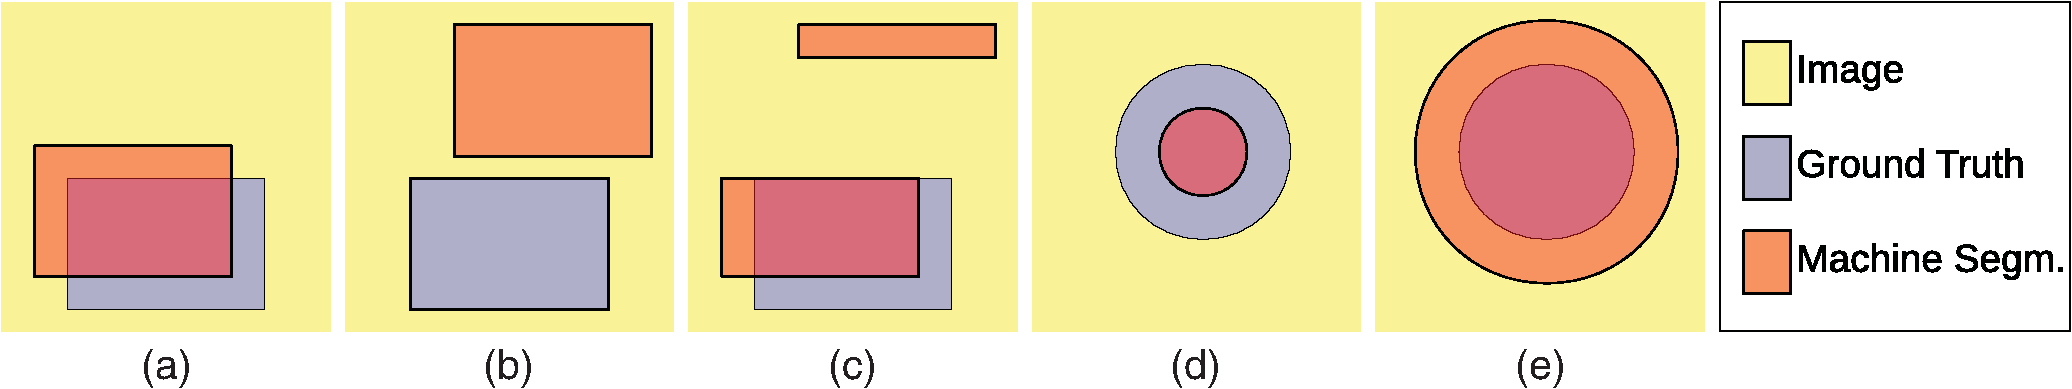
\includegraphics[width=\linewidth]{../figures/segmentation-cases-1.png}
%   \caption{Figure from~\cite{boundary-overlap-metrics} illustrating cases of segmentation to aid with explanation of set-backs of certain evaluation metrics}
%  \label{fig:segmentation-cases-1}
% \end{figure}

% \begin{itemize}
%   \item Classification Based (Section~\ref{sect:classification-based}) and Spatial Overlap Based (Section~\ref{sect:spatial-overlap-based}) are similar; they are concerned with the number of correctly classified or misclassified voxels without taking into account their spatial distribution. Here, Figure~\ref{fig:segmentation-cases-1}(a) and Figure~\ref{fig:segmentation-cases-1}(c) would achieve similar results despite Figure~\ref{fig:segmentation-cases-1}(a) being locally bound to a better area.
%   \item With Haussdorf Distance (Section~\ref{sect:surface-based}) output segmentations generated by Figure~\ref{fig:segmentation-cases-1}(d) and Figure~\ref{fig:segmentation-cases-1}(e) will result in the same score, which is not favorable in a radiotherapy planning environment where an organ-at-risk is involved.
%   \item Figure~\ref{fig:segmentation-cases-1}(b) would score flawlessly when using volumetric score estimation, however, it doesn't take into acount spatial placement, which makes this measurement rather poor when used individually.
% \end{itemize}

% \section{Estimated Editing Based}\label{sect:surface-dice}

% \begin{warning}
%   This is a quotation from this paper,~\cite{Sherer2021-le}, however, it is referencing a paper of its own. Shall I reference the original paper or are 'linked' references OK?
% \end{warning}

% It is difficult to select a measurement which can reflect a clinicians acceptability score. A study found that there was a lack of correlation between a geometric index and expert evaluation, with the JAC score having a 13\% False Positive Rate. The conclusion of the study summarised that scores such as JSC and volumetric DSC, ``provide limited clinical context and correlation with clinical or dosimetric quality''~\cite{Sherer2021-le}.

% % Because of the clinical context of evaluating the segmentation by a machine, it may sometimes be helpful to define a performance metric as the ``fraction of the surface that needs to be redrawn''~\cite{Nikolov2021-xe} since models at this point require manual review to avoid automation bias (Section~\ref{sect:using-the-tool}). For larger structures, this method is useful it doesn't assign a lot of weight on the large trivial internal volume which accounts for a much larger proportion of the score.

% \subsection{Surface DSC}\label{sect:surface-DSC}

% The study at~\cite{Sherer2021-le} helped drive an initiative to combine aspects of Surface Based evaluation (Section~\ref{sect:surface-based}) and Spatial Overlap Based evaluation (Section~\ref{sect:spatial-overlap-based}) into a Surface DICE. This assesses the specified tolerance instead of the overlap of the two volumes.

% \begin{figure}[H]
%   \centering
%   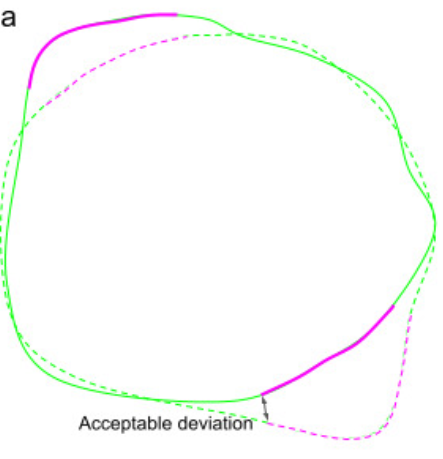
\includegraphics[width=0.3\linewidth]{../figures/Surface-dice.png}
%   \caption{Taken from~\cite{Nikolov2021-xe}. Illustrates the computation of the surface DICE, where the continuous line is the predicted surface and the dashed line is the ground truth. The black arrows show the maximum deviation tolerated without penalty; therefore, in pink is the unacceptable deviations and green otherwise.}
% \end{figure}

% We can formulate the Surface DSC score in a mathematical definition~\cite{Sherer2021-le}.

% \begin{equation*}
%   \text{Surface DSC} = \frac{|S_p \cap B_{g,\tau}| + |S_g \cap B_{p,\tau}|}{|S_p| + |S_g|}
% \end{equation*}

% Which provides a measure of the agreement between just the surfaces of two structures above a clinically determined tolerance parameter, $\tau$. Here, $B_{p,\tau}$ represents the  boundary region of the predicted surface within a maximum margin of deviation $\tau$ and similarly for $B_{g,\tau}$ for the ground truth.

% \subsection{Added Path Length}

% In a similar spirit, the APL was proposed as a score to predict ``the path length of a contour that has to be added''~\cite{APL}. This is achieved similarly by considering the number of added voxels required between the prediction and the gold standard with no regard to tolerance as a pose to Surface DSC (Section~\ref{sect:surface-DSC})

% \begin{warning}
%   For future reference, \textit{\href{https://stackoverflow.com/questions/73286639/how-to-calculate-added-path-length-apl-image-segmentation-metric}{stack overflow discussion}}

%   Implementation of surface DSC and APL: \textit{\href{https://github.com/pyplati/platipy/blob/master/platipy/imaging/label/comparison.py}{source code}}
% \end{warning}

% \section{Summary}

% This is why we settle at the Surface DSC (Section~\ref{sect:surface-dice}) which prioritizes deviation along boundary to a certain degree while measuring the fraction of the surface that needs to be redrawn, thus favouring a more conservative prediction of Figure~\ref{fig:segmentation-cases-1}(d) instead of (e).

% For the purpose of this project, we shall select a evaluation measurement which is more bias towards conservative boundary estimates to not touch the organs at risk. This choice was in-part influenced by the clinician's review pipeline; it would easier to correct Figure~\ref{fig:segmentation-cases-1}(d) instead of (e) because correcting the latter would likely take a considerable amount of time as it would require redrawing almost all of the boundary, whereas the former could be corrected much faster~\cite{Nikolov2021-xe}.

% \begin{figure}[H]
%   \centering
%   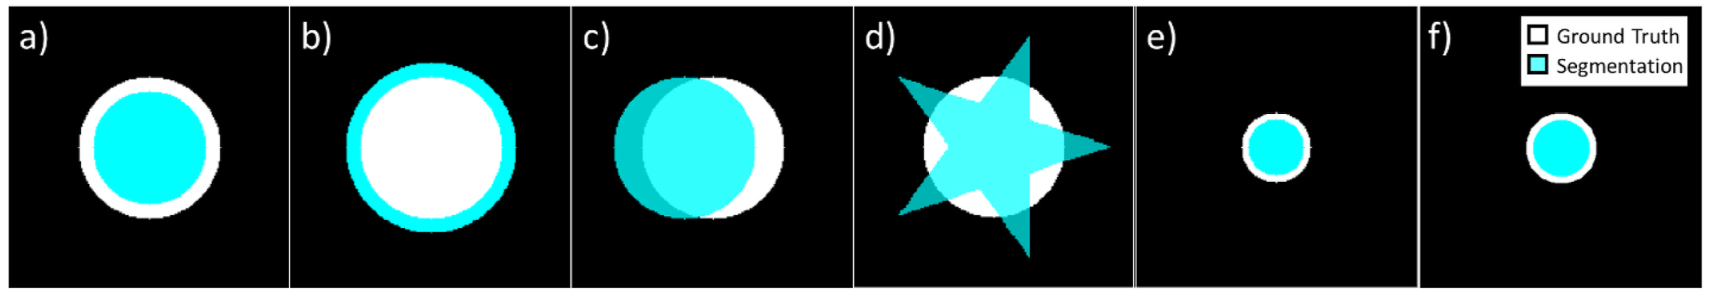
\includegraphics[width=\linewidth]{../figures/segmentation-cases-2.png}
%   \caption{Figure from~\cite{evaluation-of-metrics-in-prostate} illustrating cases of segmentation to aid with explanation of set-backs of certain evaluation metrics}
%  \label{fig:segmentation-cases-2}
% \end{figure}

%%%%%%%%%%%%%%%%%%%%%%%%%%%%%%%%%%%%
% \chapter{Proposal}\label{sect:proposal}

% \section{Baseline Results}\label{sect:baseline-results}

% \begin{warning}
%   TODO for all
% \end{warning}

% \subsection{nnU-Net}\label{sect:results-nnu-net}

% \subsection{Total Segmentator}\label{sect:results-totalseg}

% \subsection{UinverSeg}\label{sect:results-universeg}

% \section{Summary}\label{sect:results-summary}


% \begin{warning}
%   Should we keep labels individual and segment them separately or should we segment it all in one shot?
% \end{warning}

% \begin{warning}
%   Solution to resolution problem, down-sample all samples or think of average?
% \end{warning}

% Advice for Transfer Learning tasks to consider:
% \begin{enumerate}
%   \item Obtain a pre-trained 'base' model. This model has been trained on extensive data and has identified general features and patterns relevant to numerous related jobs.
%   \item Identify the transfer-layers. These capture generic information relevant to the new task as well as the previous one. These are 'frozen' in the final deliverable (see Figure~) as we want to preserve the low-level learnt features. A layer is frozen or 'fixed' when it is no longer avaialble for training, hence the weights of these layers will not be avaialble for updates.
%   \item Fine-tune and retrain the remaining layers. The goal is to preserve the knowledge from the pre-training while enabling the model to modify its parameters to better suit the demands of the current assignment. We can either
%       \begin{itemize}
%           \item freeze a few layers of the pre-trained model and train other layers on our new dataset for the new task
%           \item or make a new model, but also take out some features from the layers in the pre-trained model and use them in a newly created model
%       \end{itemize}
%   \item The number of frozen layers depend on how much you want to inherit from the pre-trained model. If the networks are significantly different (i.e. use a human face detector to detect cars) selecting many layers for freezing will not only give low level features but also give high-level features like nose, eyes, etc which are useless for new dataset (car detection). Therefore, in this case you only copy the low level features~\cite{geeks-transfer-learning}.

%   \item \textbf{Set the learning rate to be low}: It is essential to utilize a lower learning rate when compiling the new model because you are training a much larger model and want to readjust the pretrained weights. If not, your model may rapidly become overfit~\cite{geeks-transfer-learning}. Furthermore, this is done for a low number of iterations for the same reasons~\cite{deep-learning-book}.
%   \item \textbf{Don't use stochastic gradient descent algorithms to the whole network}; it is much more efficient to send the new training data once through the fixed pre-trained network so as to evaluate the training inputs in the new representation. Iterative gradient-based optimization can then be applied just to the smaller network consisting of the final     layers.
%   \item If a transfer method actually decreases performance, then negative transfer has occurred.
%   \item Eaton and DesJardins ``propose choosing from among candidate solutions to a source task rather than from among candidate source tasks. Their setting is multi-resolution learning, where a classification task is solved by an ensemble of models that vary in complexity. Low-resolution models are simple and coarse, while higher-resolution models are more complex and detailed''~\cite{torrey-handbook}.
%   \item Given multiple candidate source tasks, it may be beneficial to use several or all of them rather than to choose just one.

%   ``Ruckert and Kramer look at inductive transfer via kernel methods. They learn a meta-kernel that serves as a similarity function between tasks. Given this and a set of kernels that perform well in source tasks, they perform numerical optimization to construct a kernel for a target task. This approach determines the inductive bias in the target task (the kernel) by combining information from several source tasks whose relationships to the target are known''~\cite{torrey-handbook}.
%   \item 
% \end{enumerate}

























% ETHICS COMPLETELY ADDED

% \chapter{Ethics}\label{sect:ethics}

% This project involves very intimate and personal information of many female patients. Researchers may collaborate with third-parties by providing anonymized data which may not be reverse engineered back to the patient.
% The lack of this effort may result in ``stigma, embarrassment, and discrimination''~\cite{health-privacy} if the data is misused.

% \section{Patient disclosures}\label{sect:patient-disclosures}

% The Royal Marsden Hospital doesn't require ``explicit consent'' for sharing collected clinical data with outside entities as long as the patient is made aware of the ways their ``de-identified/anonymized'' data may be used ~\cite{royal-marsden-privacy-note}. Formalities are also arranged with Imperial Collage's Medical Imaging team such as acting as ``ethical data stewards''~\cite{ethics-imaging-AI}. Without such disclosure and anonymisation of data, patients may be reluctant to provide candid and complete disclosures of their sensitive information, even to physicians, which may prevent a full diagnosis if their data isn't maintained in an anonymous fashion.

% The MIRA team acts as responsible data stewards by storing anonymized data within a folder on the college network. All provided data was anonymized by the Royal Marsden Hospital and sent to team MIRA in the \texttt{NIfTI} file format which discloses no personal identifiable information, as defined by GOV website~\cite{gov-gdpr}. This folder contains security measures which limit the availability of data only to those with specific access rights. Furthermore, operating on the preamble of de-identified data further reduces individual patient risk in the event that data is ever brought outside the confines of this folder.

% \section{Using the tool}\label{sect:using-the-tool}

% The applications of this tool bode well in the healthcare ecosystem as the community slowly realizes the importance of AI-powered tools for the next generation of medical technology. Radiology has been one application that has been most welcoming of the new advances in technology as there is potential for substantial aid by reducing manual labor, increasing precision and freeing up the primary care physician's time~\cite{overview-of-ai-medicine}.

% Yet, it is too early to take result the medical tool as gospel. For current cervical radiotherapy delineation tools, only 90\% of the output is considered as acceptable for clinical use~\cite{auto-delineation-cervical-cancer-development}. The remainder therefore has the potential to cause more harm than good if not checked properly. For example, overlap of a PTV onto an organ-at-risk may invoke a cascade of negative effects for the patient. A potential cause may be the lack of multivariate analysis, where an oncologist would need to consider a variety of data, whereas this model only considers a single point of evidence (results of an imaging modality).

% Clinicians can fall into the trap of automation-bias as AI becomes more common place in clinical environments~\cite{automation-bias}. However, many models of this age codify the existing bias in common cases, which often will fail those patients who do not fit the expectations of the majority. Therefore, a degree of supervision required from physicians has to be established if this tool is to be used in practice. Oncologists will be required to reverse-engineer results of the `black-box' to verify why a decision has been made. Secondly, the responsible party for incorrect decisions made by DL tools should also be determined~\cite{AI-in-cancer-diagnosis-era}.


%% bibliography
\bibliography{../.latex-templates/references}

\end{document}